% Standalone render of generated_intraday_dh/table_rule_by_strategy_dh_holdclose_0935.tex
% Build: pdflatex -interaction=nonstopmode rule_by_strategy_dh_holdclose_0935.tex
\documentclass{article}
\usepackage[landscape,margin=0.5in]{geometry}
\usepackage{booktabs}
\usepackage{amsmath}
\usepackage{graphicx}
\pagestyle{empty}

\begin{document}
\begin{center}
\textbf{0DTE nearest-OTM straddle: per-rule return summary, entry 09:35 ET, held to cash-settle, models compared on the same 866 days}\\[1.5ex]
% AUTO-GENERATED by writeup/make_rule_by_strategy_intraday_tex.py -- do not edit.
% Source: results/atm_straddle_intraday/rule_by_strategy/0935/rule_by_strategy_*.csv
\begingroup\small\setlength{\tabcolsep}{3.6pt}
\begin{tabular}{lrrrrrrrrrrrr}
\toprule
& $n$ & mean & std & min & max & skew & ex.\ kurt & $t$ & Sharpe$_{\mathrm{clk}}$ & $n_{\mathrm{buy}}$ & \%buy & Sharpe$^{\times}_{\mathrm{clk}}$ \\
\midrule
\multicolumn{13}{l}{\emph{Short volatility (always short)}} \\
all models (no forecast) & 863 & 0.076 & 0.385 & -3.97 & 0.90 & -2.97 & 23.37 & 5.76 & 3.11 & 0 & 0.0 & 2.44 \\
\midrule
\multicolumn{13}{l}{\emph{$\mathrm{sign}(s)$ ($\pm 1$ on the sign of $s$)}} \\
baseline (HAR + calendar OLS) & 863 & 0.042 & 0.391 & -3.47 & 3.97 & -0.00 & 19.95 & 3.16 & 1.71 & 289 & 33.5 & 1.04 \\
block-diagonal ridge & 863 & 0.017 & 0.392 & -3.47 & 3.97 & 0.23 & 19.53 & 1.26 & 0.68 & 405 & 46.9 & 0.02 \\
block-diagonal ridge, without the FOMC columns & 863 & 0.015 & 0.393 & -3.47 & 3.97 & 0.24 & 19.52 & 1.14 & 0.62 & 408 & 47.3 & -0.04 \\
LightGBM$^{\dagger}$ & 863 & 0.037 & 0.391 & -3.47 & 3.97 & 0.05 & 19.83 & 2.80 & 1.51 & 322 & 37.3 & 0.85 \\
XGBoost$^{\dagger}$ & 863 & 0.040 & 0.391 & -3.47 & 3.97 & 0.04 & 19.89 & 2.99 & 1.61 & 306 & 35.5 & 0.95 \\
lasso (causally tuned)$^{\dagger}$ & 863 & 0.028 & 0.392 & -3.47 & 3.97 & 0.16 & 19.65 & 2.09 & 1.13 & 372 & 43.1 & 0.46 \\
lasso ($\alpha=10^{-4}$) & 863 & 0.019 & 0.392 & -3.47 & 3.97 & 0.22 & 19.54 & 1.39 & 0.75 & 400 & 46.3 & 0.09 \\
elastic net (causally tuned)$^{\dagger}$ & 863 & 0.023 & 0.392 & -3.47 & 3.97 & 0.11 & 19.61 & 1.74 & 0.94 & 384 & 44.5 & 0.28 \\
\bottomrule
\end{tabular}
\endgroup

\end{center}
\vspace{1ex}
\begin{center}
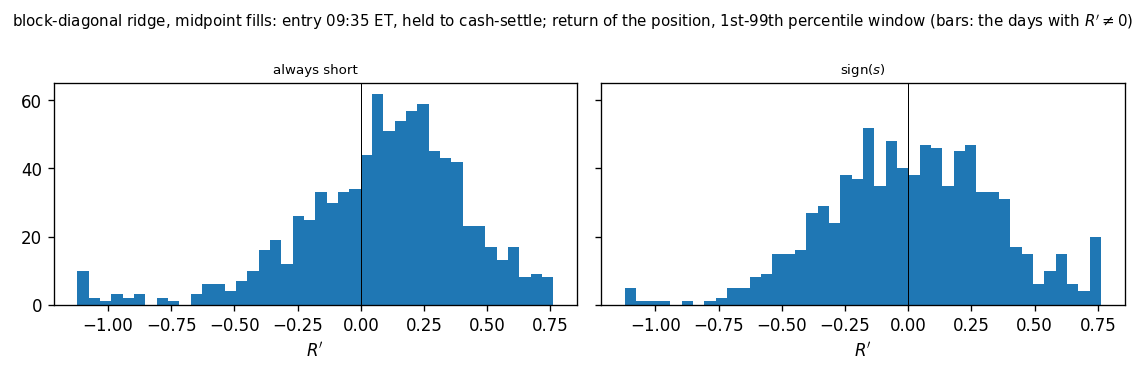
\includegraphics[width=0.27\textwidth]{../results/atm_straddle_intraday_holdclose/rule_by_strategy_dh/0935/rule_hists_blk2_0935.png}\par\smallskip
\small Distribution of the return of the position taken at 09:35 ET, block-diagonal ridge forecast, one panel per rule (returns inside their 1st--99th percentile window).
\end{center}
\vspace{1ex}
\noindent\small One trade a day: enter the nearest-OTM straddle at 09:35 ET, hold those strikes to the official close, and delta-hedge at 10:00 and then every 30 minutes. 863 expiration days (the other 3 of the deck's 866 days have no quoted straddle at this stamp), 2020-01-03 to 2024-04-30 (the deck's frame). Fills are at the quoted midpoint everywhere except the last column, which is the same rule at the crossed spread: entry at the touch (the ask when long, the bid when short) and cash-settle at the official close (no exit spread). \textbf{The 09:35 entry.} The first stamp of the session is 09:35, and no forecast bar starts there: the forecasts are for half-hour bars 09:30--10:00, 10:00--10:30, and so on. The forecast used at 09:35 is therefore the one issued at 09:30 for the 09:30--10:00 bar, which is known five minutes before the entry. It covers 09:30--10:00 while the straddle is entered at 09:35; it is used as issued, with no rescaling for the five minutes. The implied side is priced the same way: its diurnal share is the 09:30--10:00 bar's share of the rest of the session, averaged over prior days only (the same expanding mean as at every other clock), and the hours to the close are the chain's, 6.42 hours (6 h 25 min). This design was fixed before the 09:35 numbers were computed.
\vspace{1ex}
\noindent\small \textbf{Straddle} here means the nearest out-of-the-money call plus the nearest out-of-the-money put, same-day expiry, bought or sold as one position. One expiration day = one return; mid fill. Every $t$ here is the plain $t=\sqrt{n}\cdot\mathrm{mean}/\mathrm{std}$, with no autocorrelation correction. ``ex.\ kurt'' is the bias-corrected sample excess kurtosis (Gaussian $=0$). The short-volatility rule takes no forecast, so it is one row for all models. \textbf{Two Sharpes.} Both multiply by $\sqrt{252}$ because an expiration day is the unit of time (same year-length as the paper). They are not the same object. On a \emph{single-clock} page, Sharpe$_{\mathrm{clk}}=(\mathrm{mean}/\mathrm{std})\times\sqrt{252}$ of that clock's series: one remaining-session short per expiration day (enter at this clock, hold those strikes to the close, delta-hedge every 30 minutes). It answers ``if I only entered at this clock, what is my annual Sharpe?'' It is \emph{not} the book's Sharpe$_{\mathrm{ann}}$. On the \emph{pooled} page, Sharpe$_{\mathrm{ann}}=(\mathrm{mean}/\mathrm{std})\times\sqrt{252}$ of $R^{day}_d=\sum_t R'_{d,t}$, the sum of the day's thirteen overlapping remaining-session books. That reserved name is the book's daily P\&L after pooling the session. The thirteen books overlap; they are not thirteen successive holds. Sharpe$^{\times}$ is the same convention at the crossed spread. Every other column is daily. $n_{\mathrm{buy}}$ is the number of expiration days with position $>0$ (always-short is 0; on the pooled page it is days the sum of the thirteen positions is positive); \%buy is $100\cdot n_{\mathrm{buy}}/n$, the notebook's column. The other column this table adds to the deck's is Sharpe$^{\times}_{\mathrm{ann}}$, the same rule's annualized Sharpe at the \emph{crossed spread} instead of the midpoint; every other column is the deck's.

\smallskip
\noindent\small Forecasts: baseline (HAR + calendar OLS); block-diagonal ridge (HAR block and exogenous block, separate penalties) on the design carrying the FOMC calendar block, and the same ridge on the earlier design without those columns, as a diagnostic row; LightGBM and XGBoost on the all-features design; lasso on the same design, causally tuned vs.\ fixed $\alpha=10^{-4}$; elastic net (causally tuned). $\dagger$ marks a column still fitted on the earlier design panel; a run of those four on the panel of record is pending. The signal is $s_t=\widehat{RV}_t-\mathrm{IV}^{2}_{\mathrm{hr}}h_t w_t$: the forecast against the implied variance of the same window. $w_t$ is the expanding mean of each prior day's remaining-session share of realized variance, $\mathrm{RV}_t/\sum_{s\ge t}\mathrm{RV}_s$ (in-fit panel history back to 2001), not the ratio of trailing clock-means. On the bars whose vendor implied volatility is a censored solver node the deck's treatment is used here too --- the volatility that reproduces the straddle midpoint, recovered by bisection over the remaining $h_t$ hours --- so every bar carries a signal and no bar sits flat. At the 09:35 entry the forecast is the one issued at 09:30 for the 09:30--10:00 bar, $w_t$ is that bar's share, and $h_t$ is the chain's hours to the close.
\end{document}
